\documentclass[10pt,aspectratio=169]{beamer}
\setbeamertemplate{navigation symbols}{}
\setbeamertemplate{headline}{}
\setbeamertemplate{footline}{}
\setbeamerfont{frametitle}{series=\bfseries,size=\large}

\usepackage{amsmath}
\usepackage{booktabs}
\usepackage{graphicx}
\usepackage{xcolor}

\definecolor{pinbg}{RGB}{224,221,204}
\setbeamercolor{background canvas}{bg=pinbg}
\setbeamercolor{normal text}{fg=black,bg=pinbg}
\setbeamercolor{frametitle}{fg=black,bg=pinbg}

\title{PIN Local Radio Control Overlay}
\subtitle{One-Slide Optimization + Control + Results Summary}
\author{}
\date{}

\begin{document}

\begin{frame}[t]{PIN Optimization, Control, and Results}
\footnotesize
\setlength{\columnsep}{1.2em}
\begin{columns}[T,onlytextwidth]
  \begin{column}{0.54\textwidth}
    {\bfseries Constrained local optimization (per radio \(i\))}\par
    \vspace{0.15em}\rule{\linewidth}{0.3pt}\vspace{0.35em}
    \begin{align*}
      \max_{\pi_\theta}\; \mathbb{E}\!\left[\sum_{t=0}^{T-1}\gamma^t r_t\right] \\
      \text{s.t.}\;\;
      PDR_t^{cmd}\ge p_{\min},\;
      L_{95,t}^{cmd}\le \ell_{\max},\;
      Drop_t^{cmd}\approx 0
    \end{align*}
    \vspace{-0.9em}
    \[
      r_t=\alpha PDR_t^{high}-\beta L95_t^{high}
      -\delta Drop_t^{high}+\zeta Deliveries_t^{high}
    \]

    \vspace{0.2em}
    {\bfseries PIN local control I/O (every 250 ms)}\par
    \vspace{0.15em}\rule{\linewidth}{0.3pt}\vspace{0.4em}
    {\scriptsize
    \textbf{Observation \(o_t^{(i)}\):} queue length by class; tx attempts/success;
    retries/ACK timeouts; drops/deliveries; p95 latency by class; collisions;
    CCA busy fraction; mean backoff.\par
    \vspace{0.35em}
    \textbf{Action \(a_t^{(i)}\):} for class \(c\in\{\text{command, voice, best-effort}\}\)
    \[
      a_t^{(i)}=\{w_c,\eta_c,\kappa_c\}_{c=1}^{3}
    \]
    \vspace{-0.65em}
    where \(w_c\) is service bias, \(\eta_c\) admission threshold, \(\kappa_c\) CW scaling.
    }
  \end{column}

  \begin{column}{0.42\textwidth}
    {\bfseries Seeded A/B demo (CSMA, 8 nodes, 1.5 s)}\par
    \vspace{0.15em}\rule{\linewidth}{0.3pt}\vspace{0.35em}
    \centering
    {\scriptsize
    \setlength{\tabcolsep}{3.0pt}
    \begin{tabular}{lrrr}
      \toprule
      KPI & Base & Ctrl & \(\Delta\) \\
      \midrule
      High PDR & 0.6995 & 0.6979 & -0.0016 \\
      High p95 (ms) & 8.9836 & 9.4497 & +0.4662 \\
      Overall PDR & 0.8193 & 0.8270 & +0.0077 \\
      Overall p95 (ms) & 36.8898 & 31.2521 & -5.6377 \\
      \bottomrule
    \end{tabular}
    }

    \vspace{0.5em}
    \raggedright\textbf{Highlight seed 202:}
    \(+\)0.0038 high-PDR, \(+\)0.0169 overall PDR,\par
    \(-\)5.5065 ms overall p95 latency.\par
    \vspace{0.45em}
    \centering
    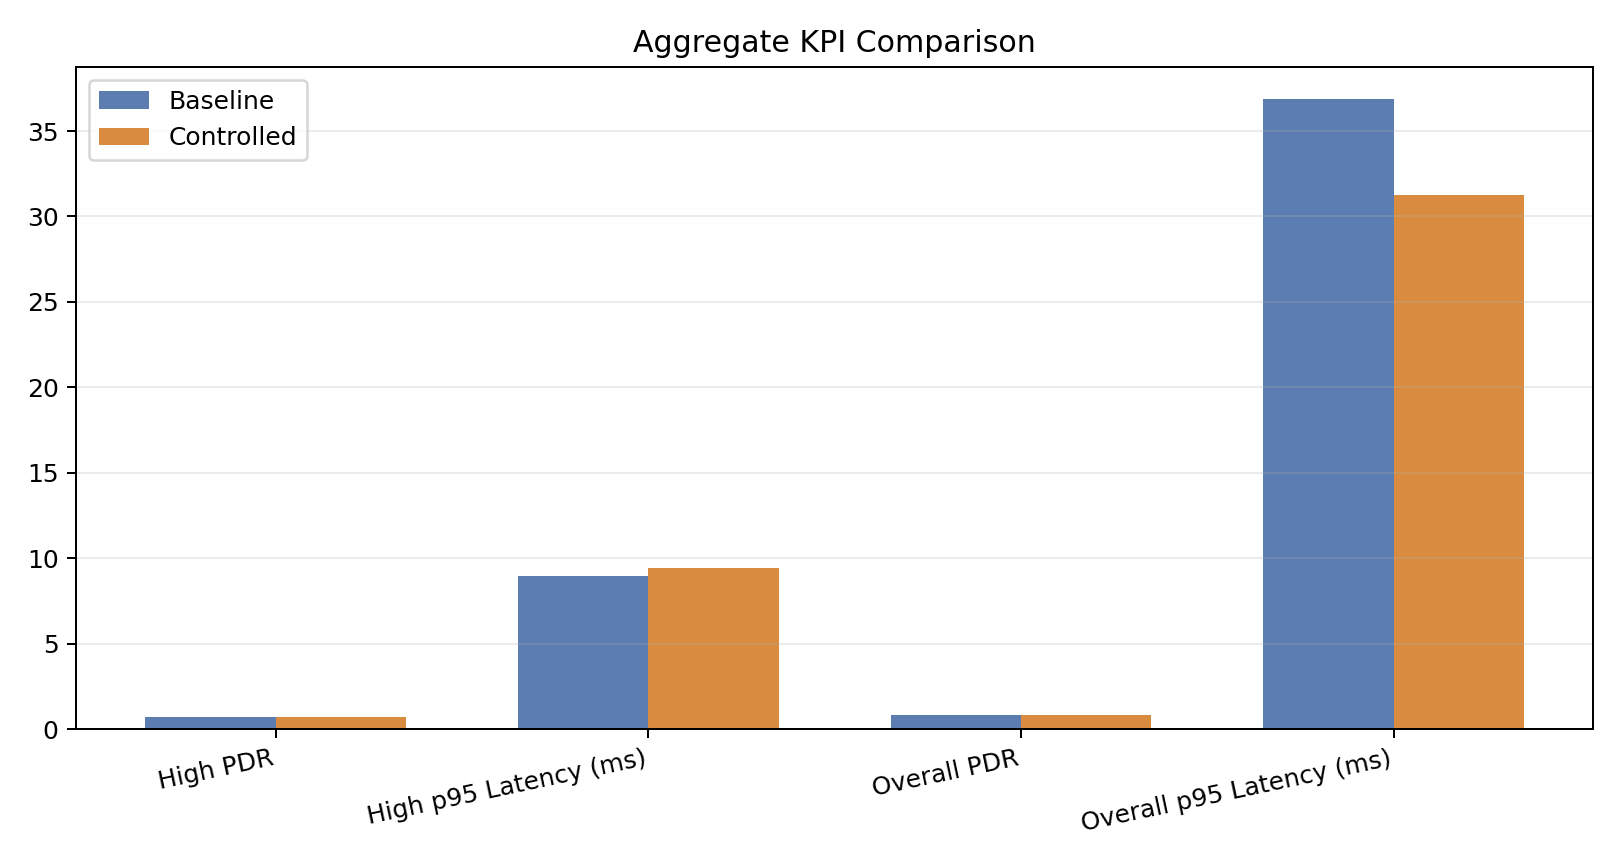
\includegraphics[width=0.94\linewidth]{figures/pin_demo/aggregate_kpi_comparison.png}
  \end{column}
\end{columns}

\vfill
\tiny Data: \texttt{pin\_demo\_metrics.json} (eval seeds 201, 202; local-only PIN overlay).
\end{frame}

\end{document}
